\documentclass[11pt, a4paper]{article}

\usepackage[utf8]{inputenc}
\usepackage[T1]{fontenc}
\usepackage{amsmath}
\usepackage{amsfonts}
\usepackage{amssymb}
\usepackage{graphicx}
\usepackage{wrapfig}
\usepackage{lmodern}
\usepackage{hyperref}
\usepackage[left=2.5cm,right=2.5cm,top=2.5cm,bottom=2.5cm]{geometry}
\usepackage{listings}
\lstset{breaklines=true}

%watermark
%\usepackage{draftwatermark}
%\SetWatermarkText{Preliminary}
%\SetWatermarkLightness{0.9}
%\SetWatermarkScale{1}

\lstdefinelanguage[markII]{Assembler}
{
    alsoletter={.\#},
    morekeywords={[1]RET, RETI, CALLI, PUSH, POP, LDI, STI, BZI, BNZI, MOV, CMP, AND, OR, XOR, ADD, SUB, INC, DEC, LSL, LSR, ROL, ROR, MVIL, MVIH, CALL, LD, ST, BZ, BNZ, MVIA},
    morekeywords={[2]\#define, \#ifdef, \#ifndef, \#endif, \#include, \#macro, \#endmacro, .CONS, .ORG, .DAT, .DS, .EXPORT, .IMPORT, .MVI},
    morekeywords={[3]R0, R1, R2, R3, R4, R5, R6, R7, R8, R9, R10, R11, R12, R13, R14, R15, SP, PC},
    morekeywords={[4]EQ, NEQ, L, LU, GE, GEU},
    sensitive=false,
    morecomment=[l]{;},
}[comments,keywords]

\author{Vladislav Mlejnecký}
\title{\huge MARK-II Reference Manual}

\begin{document}

\pagenumbering{gobble}
\maketitle
\vfill
\begin{figure}[h]
\centering
\begin{minipage}{.06\textwidth}
  \centering
  \includegraphics[width=.9\linewidth]{img/lic/cc.png}
\end{minipage}
\begin{minipage}{.06\textwidth}
  \centering
  \includegraphics[width=.9\linewidth]{img/lic/by.png}
\end{minipage}
\begin{minipage}{.06\textwidth}
  \centering
  \includegraphics[width=.9\linewidth]{img/lic/nc.png}
\end{minipage}
\end{figure}
\begin{flushleft}
    \copyright  2017 Vladislav Mlejnecký - v.mlejnecky@seznam.cz.
    This work is licensed under the Creative Commons Attribution-NonCommercial 4.0 International License.
    To view a copy of this license, visit \url{http://creativecommons.org/licenses/by-nc/4.0/}
\end{flushleft}
\newpage
\pagenumbering{roman}
\tableofcontents
\newpage
\listoffigures
\newpage
\listoftables
\newpage
\pagenumbering{arabic}

\section{Introduction}

MARK II is simple SoC written in VHDL for synthesization into Altera Cyclone
FPGA. SoC consist of simple RISC like CPU and a few peripherals. There is also
full featured toolchain for writing programs that can run on MARK-II CPU.

CPU is 32 bits wide and following Von Neumann architecture, can address up to
$2^{24}$ words, has 16 interrupt sources, 16 registers including three special
ones.

To the CPU can be connected memory mapped peripherals, following peripherals
are available: UART, PS/2, VGA driver, general purpose timers, system timer,
GPIO, onchip RAM and ROM and interrupt controller.

Thanks to toolchain, you can write programs in human way. Toolchain consist of
Assembler, Linker, Emulator, Disassembler, Loader and ldm2mif converter. There is
also backend for vbcc so you can compile your C programs too.

This document is reference guide for MARK-II CPU. But because this project is really
complex and still it is one man show, some informations in this manual can be
outdated. If you are get stuck on something, please see source codes or
contact author.

MARK-II is home project, created just for fun. There isn't any main goals
except one, have fun from coding. As home fun project, is mostly licensed under
MIT license to be free for everybody to try run it. But due to complexity there
are some parts that is licensed under another license, for example vbcc front
end.

Anyway, some goals exist, but they are more like "I want to try ..." rather than
"I have to ...", these goals are changing in time and they are following topics
that I want to explore.


\section{System overview}

Heart of SoC is CPU. The CPU is only one master on the system bus and it control
all communication on this bus. To the CPU is directly connected interrupt
controller.

Bus consist of 24b address, 32b MOSI data, 32b MISO data, clock, reset, write,
read and ack signals. There is also 32b bus for interrupts.

All the peripherals are connected to the system bus, CPU select peripheral to
communicate with through address. Peripheral control ack signal to say to CPU
"data is ready for read" when CPU want read data, or "data is written" when CPU
want write data. This allow slower peripheral to cooperate with CPU, CPU simply
wait for them.

Some peripherals have special pins, these are commonly connected to the top
level entity pins, but there are few that are connected internally, for example
pll outputs.

CPU have multiple clock domain. At this moment there are two domains, one is for
VGA pixel clock and another is for rest SoC (CPU/Timers/UARTs and so on).
Clocks are generated by pll from 50MHz input. 50MHz was selected because 50MHz
oscillators are common on the Terasic FPGA boards.

\begin{wrapfigure}{L}{0.6\textwidth}
    \centering
    \includegraphics[width=0.55\textwidth]{img/MARK_II.png}
    \caption{MARK-II system architecture}
    \label{fig:sysarch}
\end{wrapfigure}

On the figure \ref{fig:sysarch} is simple high level schematic of MARK-II system architecture,
you can see bus, CPU and all units. PLL and clock control are only two units
that are not connected to the main BUS. They are don't need any configuration.

PLL unit is generating predefined frequencies, and clock control unit is
generating control signals for clock dividers in other modules.

Another special module is interrupt control unit. It is connected directly to
the CPU and also connected on system BUS. Interrupt control unit have interrupt
sources that are connected to the others modules such are Timers or UARTs.

\subsection{Memory map}

In the table \ref{tab:memory_map} is simple memory map. There are listed all
peripherals implemented in MARK II SoC. Each peripheral have one or more registers at different
addresses.

Lets say, GPIO have 0x00100 as base address, one of the GPIO register
is DDRB register with offset +3, so address of DDRB register is 0x00103. For
informations about individual register please see corresponding peripheral sections.

\begin{table}[h]
    \centering
    \begin{tabular}{|l|l|l|l|l|}
        \hline
        \textbf{Peripheral} & \textbf{Base} & \textbf{Size} & \textbf{End} & \textbf{Note}                                  \\ \hline
        ROM                 & 0x000000      & $2^{8}$       & 0x0000FF     & Read only memory                               \\ \hline
        GPIO                & 0x000100      & $2^{2}$       & 0x000103     & General purpose inputs and outputs             \\ \hline
        System Timer        & 0x000104      & $2^{1}$       & 0x000105     & 24b system timer                               \\ \hline
        Interrupt driver    & 0x000108      & $2^{0}$       & 0x000108     & Enable and disable interrupts                  \\ \hline
        PS2 Keyboard        & 0x000109      & $2^{0}$       & 0x000109     & PS2 interface driver                           \\ \hline
        Timer 0             & 0x000110      & $2^{2}$       & 0x000113     & General purpose timer 0                        \\ \hline
        Timer 1             & 0x000114      & $2^{2}$       & 0x000117     & General purpose timer 1                        \\ \hline
        Timer 2             & 0x000118      & $2^{2}$       & 0x00011B     & General purpose timer 2                        \\ \hline
        Timer 3             & 0x00011C      & $2^{2}$       & 0x00011F     & General purpose timer 3                        \\ \hline
        UART 0              & 0x000120      & $2^{2}$       & 0x000123     & Serial port 0                                  \\ \hline
        UART 1              & 0x000124      & $2^{2}$       & 0x000127     & Serial port 1                                  \\ \hline
        UART 2              & 0x000128      & $2^{2}$       & 0x00012B     & Serial port 2                                  \\ \hline
        on-chip RAM0        & 0x000400      & $2^{10}$      & 0x0007FF     & Simple onchip RAM - fastest RAM in SoC         \\ \hline
        VGA                 & 0x001000      & $2^{13}$      & 0x001FFF     & VGA GPU - text mode output 80x30 chars         \\ \hline
        on-chip RAM1        & 0x100000      & $2^{13}$      & 0x101FFF     & Simple onchip RAM - fastest RAM in SoC         \\ \hline
    \end{tabular}
    \caption{Memory map}
    \label{tab:memory_map}
\end{table}

\subsection{Interrupt sources}

In the table \ref{tab:intsources} are listed all interrupt vectors. Destinations
addresses of interrupts are hardwired into CPU and cannot be changed. All
interrupts are mascable using interrupt controller.

Support for nested interrupts isn't implemented. When one interrupt come, CPU
will jump into interrupt service routine and until RETI instruction is executed,
another interrupt cannot be raised. Anyway, when an interrupt is active, another
one is then put into queue.

\begin{table}[h]
    \centering
    \begin{tabular}{|l|l|l|}
        \hline
        \textbf{Int number} & \textbf{Peripheral} & \textbf{Purpose}                \\ \hline
        0                   & SWI                 & Software interrupt              \\ \hline
        1                   & System Timer        & SysTim compare match / overflow \\ \hline
        2                   & -                   & -                               \\ \hline
        3                   & -                   & -                               \\ \hline
        4                   & -                   & -                               \\ \hline
        5                   & -                   & -                               \\ \hline
        6                   & -                   & -                               \\ \hline
        7                   & -                   & -                               \\ \hline
        8                   & UART0               & Serial port 0                   \\ \hline
        9                   & UART1               & Serial port 1                   \\ \hline
        10                  & UART2               & Serial port 2                   \\ \hline
        11                  & PS2 Keyboard        & Byte received                   \\ \hline
        12                  & Timer 0             & Timer compare match / overflow  \\ \hline
        13                  & Timer 1             & Timer compare match / overflow  \\ \hline
        14                  & Timer 2             & Timer compare match / overflow  \\ \hline
        15                  & Timer 3             & Timer compare match / overflow  \\ \hline
    \end{tabular}
    \caption{List of all interrupt sources}
    \label{tab:intsources}
\end{table}

\subsection{Brief peripheral informations}

\subsubsection{On-chip ROM}

On-chip ROM is small memory for your program, it can be initialized with content
 at the synthesizing design into FPGA. This memory have only 1kB (256 words).

\subsubsection{GPIO}

Really simple peripheral but widely used. GPIO consist from two eight bit ports.
 Each pin in port can be configured as output or input.

\subsubsection{SysTimer}

Simple 24b timer. It will generate interrupt on compare match and then start
counting from zero.

\subsubsection{Interrupt driver}

Simple interrupt controller allowing disabling individual interrupts and
setting theirs address. Also take care about priorities.

\subsubsection{UART}

Universal asynchronous receiver/transmitter is intended for serial communication
with many devices like computers, another micro-controllers, modules and so on.
It has build in baud rate generator and also provide configurable interrupt sources.

\subsubsection{Timers}

Basic 16b timers with PWM output generation and interrupts. Timer can generate
interrupt on compare match like SysTimer, on overflow or on both.

\subsubsection{On-chip RAM}

Bigger place for data and program. CPU can run program from there too because
it is designed as Von Neumann architecture. RAM have 4kB in size, so there are
1024 words. This RAM is faster than external, you can use it for accelerate your
programs by storing them here, or at least, store variables here.

\subsubsection{PS2 driver}

With PS2 driver you can connect keyboard to the SoC. This driver is really
simple and it is able only to receive data from keyboard. It will also generate
interrupt when data from keyboard come.

\subsubsection{VGA driver}

VGA driver is useful form of output. It work in text mode with resolution 80x30
characters. Each character have size 8x16 pixels. This is 640x480@73hz effective
resolution. VGA driver also support colors, you can specify color for foreground
(character) and for background.


\section{CPU core architecture}

In this section reader can found informations about CPU core. For example,
count of registers, instructions, memory organization and so on.

\subsection{CPU Features}

\begin{itemize}
    \item $2^{24}$ word addressed memory
    \item 16 registers for both integers and floats
    \item Integer ALU with fast multiplier and divider
    \item Fast FPU with single precision format
    \item Fast barrel shifter
    \item Almost all instructions are done in 3 cycles (Load, decode and execute)
\end{itemize}


\subsection{Registers}

\begin{table}[h]
    \centering
    \begin{tabular}{|l|l|l|l|}
        \hline
        \textbf{Register name} & \textbf{Purpose} & \textbf{Register name} & \textbf{Purpose} \\ \hline
        R0                     & zero register    & R8                     & 32b GPR          \\ \hline
        R1                     & 32b GPR          & R9                     & 32b GPR          \\ \hline
        R2                     & 32b GPR          & R10                    & 32b GPR          \\ \hline
        R3                     & 32b GPR          & R11                    & 32b GPR          \\ \hline
        R4                     & 32b GPR          & R12                    & 32b GPR          \\ \hline
        R5                     & 32b GPR          & R13                    & 32b GPR          \\ \hline
        R6                     & 32b GPR          & R14                    & Program counter  \\ \hline
        R7                     & 32b GPR          & R15                    & Stack pointer    \\ \hline
    \end{tabular}
    \caption{List of registers}
    \label{tab:registers_list}
\end{table}

In the table \ref{tab:registers_list} are listed all CPU registers, including
special ones.

GPR mean general purpose register, these registers are 32bit wide.
Zero register is one of special registers, it always contain zero.
You can write there whatever you want, but always read zero. Program
counter (PC) and Stack pointer (SP) are implemented like any others
registers but they are holding actual address in program and actual
address of top of stack.

There is no limitation in register usage in instructions. Every
instruction can work with every register include PC and SP. There is
no register windows, banks or something like that.

\subsection{Instruction set architecture}

There is only quick explanation of meaning individual instruction. If you want
to see binary format, plese see file /doc/isa.ods.

\subsubsection{Program control instructions}

These instruction control program flow. In this group are instruction RET,
RETI, CALLI, BZI, BNZI, CALL, BZ, BNZ and SWI.

Instruction RETI is intended for returning from interrupt service routine. It
is necessary inform interrupt driver about completing the ISR. So, this is
reason why there is RETI.

Instruction RET, CALL and CALLI are for implementing subroutines. Instruction
CALL is similar to CALLI, both call subroutine and store return address into
stack. But instruction CALL excepting absolute address of subroutine.
Instruction CALLI, on the another hand, excepting register where the subroutine
address is stored. Instruction RET will take return address from stack and
continue normal program execution.

There are also instruction for conditional jumps. They are BZI, BNZI, BZ and
BNZ. BZ mean "branch zero" and BNZ mean "branch nonzero", suffix I mean where
address to jump is stored. If there is I in instruction, address is stored in
some register, instruction without I have address in their instruction word.

There isn't any flags for conditional jumps, for example, instruction BZ jump
when in specified register is zero, if there is another value, it will continue
without jumping.

SWI instruction is quiet special one. It is used to generate software interrupt.
This can be used in implementation of operating system to transfer control from
user space program to the kernel.

\subsubsection{Memory instructions}

These instruction work with memory. They are LD, LDI, ST, STI, PUSH and POP.

PUSH and POP are instruction for stack operation. PUSH save data from specified
register into stack and decrement stack pointer. POP instruction increment
stack pointer and then store data from stack into specified register.

Instruction LD and LDI load data from memory into specified register. Memory is
organized as 32b words and these instruction work only with 32b words.
Instruction LD have address in it's instruction word and LDI use address from
specified register.

Instruction ST and STI are similar to LD and LDI, but they are load data into
memory.

\subsubsection{Data move instructions}

Instruction that are intended for moving data. There are only four instruction
of this type. First is MOV. MOV instruction move data from one register into
another. Actually, copy from one register into another.

Another two instruction from this group are MVIH and MVIL. Both are intended
for loading immediate values into register, but because there are 32bit
register, instruction are 32bit wide and there have to be space for opcode in
instruction word, MVI instruction is splitted into MVIH and MVIL. MVIL will
load lower 16b into specified register and MVIH upper 16bit.

Last instruction for moving is MVIA. MVIA is similar to MVIL and MVIH, but
constant for loading is 24bit wide. Because address bus of MARK II CPU is 24bit
wide, this instruction is perfect for loading address into registers.

\subsubsection{Computation instructions}

These instruction are intended for computation on the data. MARK II CPU use
three operand arithmetic, so you have to specify three register, two for
operand, and one for result. But, there are also few instruction where only one
operand is used, for example increment instruction.

CPU is able to do basic bitwise operations, concretely AND, OR, XOR and NOT.
There are also ADD and SUB instruction for adding and subtracting, MUL and MULU
for signed and unsigned multiplication, DIV and DIVU for signed and unsigned
integer division, REM and REMU for signed and unsigned integer division remainder.

CPU also have floating point unit. In order to make computation on floats there
are instruction FADD, FSUB, FDIV and FMUL for adding, subtracting, division
and multiplication.

Instructions INC and DEC are used for incrementing and decrementing registers,
these instruction use only two operands, one for input operand and second for
result.

There are also shifting instructions LSL, LSR, ROL, ROR, ASL and ASR. LSL for
logical shift to left, LSR for logical shift to right, ROL for rotate to left,
ROR for rotate to right, ASL for arithmetic shift left and ASR for arithmetic
shift right. You can also specify distance from 0 to 31. All shifts and rotations
are done using single cycle barrel shifter.

\subsubsection{Special instructions}

Currently there is only one special instruction and that is CMP. This
instruction is mandatory for branching. With this instruction you can compare
two register with specified comparison type and store 1 if "expression" is true
or 0 if false, into specified register.

\subsubsection{More informations}

You can find more informations about instruction format in document called
MARK-II Instruction Set Architecture.

\subsection{Memory organization}

CPU can address up to $2^{24}$ words, whole memory space is linear. Everything
is in one memory space, there is nothing like IO space, program space, data
space. MARK II CPU following Von Neumann scheme, so program and also data is in
one space. Peripherals and IO devices should be mapped there too.

There are two instruction for working with memory. One is LD for reading from
memory, and second is ST for writing into memory. Both instruction can use
absolute addressing mode (address is part of instruction) or indirect
addressing with register (address is stored in register).

\subsubsection{Stack}

Stack is used for storing returning address when calling subroutines or
interrupts. It grow from up to down. So, you should set SP at end of ram.

You can also use stack for storing your variables/registers etc. There is two
special functions for that.

\begin{itemize}
    \item \textbf{PUSH} - store data into stack and decrement SP
    \item \textbf{POP} - take data from stack and increment SP
\end{itemize}

\subsection{Interrupts}

Interrupt vectors are address in memory where the CPU will jump when interrupt
occur. All addresses can be found in the table \ref{tab:intsources}. When
interrupt occur CPU will do following:

1. complete actual instruction
2. increment PC (PC always have to point to next instruction)
3. store PC into stack and decrement SP
4. jump into interrupt vector

There is only two words for every vector. This is enough only for code like this:

\begin{lstlisting}[language={[x86masm]Assembler}, frame=single]
    .ORG UART1_RX_VECTOR
        CALL UART1_RX_ISR
        RETI
\end{lstlisting}

Instruction RETI is mandatory. It will inform interrupt driver that ISR is
completed and CPU is ready to take another interrupt. There is no support for
nested interrupts. When first interrupt come, another have to wait.


\section{Peripherals}

\subsection{RAM}

Simple and fast memory. You can store your data there, you can also run program
from there.

Internal RAM is organized as 32bit wide words and is implemented with internal
SRAM block memory in FPGA. Thus is really fast. It is fastest memory what you
can use (of course, except registers).

\subsection{ROM}

Simple memory for program store. CPU can read program from this but it is not
able to write data there.

Memory is implemented in same way as RAM, but write signals is not present
there. Content of ROM is specified in ".mif" memory initialization files. These
files are used during synthesis of SoC into FPGA.

\subsection{GPIO}
Simple peripheral, two 8bit input/outputs ports. Function is similar
to AVR ports, there is two register, DDR and PORT, logical one in DDR
set this pin as output, value written into right bit of PORT register
will be on pin. When logical zero in in DDR register, CPU can read
values what are connected to the pins through PORT register.

\subsection{UART}

\subsection{Interrupt driver}

\subsection{Timer}

\subsection{System timer}

\subsection{VGA driver}

\subsection{PS2 driver}

\subsection{ROM}

Simple memory for program store. CPU can read program from this but it is not
able to write data there. By default, in rom0 is stored serial port loader and
CPU start execution there.

\subsubsection{Function}

Memory is implemented in same way as RAM, but write signals is not present
there. Content of ROM is specified in ".mif" memory initialization files. These
files are used during synthesis of SoC into FPGA.

Usage is straightforward, write data with LD instruction to address that belong
to RAM.


\subsubsection{Hacking}

At this moment, there is any simple way to change size of ROM. It is hard coded
to 256 words. In order to change it you have to modify chip select generator,
instance of lpm\_rom and mif.

Anyway, you can change memory initialization file quit simply. Just replace
"rom.mif" file in the /fpga/src/rom/ directory. New file should be organized
as 256x32bit.

\subsection{RAM}

Simple and fast memory. You can store your data there, you can also run program
from there.

\subsubsection{Function}

Internal RAM is organized as 32bit wide words and is implemented with internal
SRAM block memory in FPGA. Thus is really fast. It is fastest memory what you
can use (of course, except registers).

Usage is really straightforward, simply write data with LD instruction to address
that belong to RAM.

\subsubsection{Hacking}

SoC can have multiple instances of RAM, as much as you want and there is
enough FPGA SRAM (M9K for Cyclone IV) block free. Formula for estimate usage
of M9K is: $ blocks = \frac{2^{ADDRESS\_WIDE}}{256} $.

You can change size of internal RAM by parameter ADDRESS\_WIDE, value for this
parameter have following meaning: $ size [words] = 2^{ADDRESS\_WIDE}$.

\begin{lstlisting}[language=VHDL, frame=single]
entity ram is
    generic(
        BASE_ADDRESS: unsigned(23 downto 0) := x"000000";
        ADDRESS_WIDE: natural := 8
    );
    port(
        clk: in std_logic;
        address: in unsigned(23 downto 0);
        data_mosi: in unsigned(31 downto 0);
        data_miso: out unsigned(31 downto 0);
        WR: in std_logic;
        RD: in std_logic;
        ack: out std_logic
    );
end entity ram;
\end{lstlisting}

As you can see, there is only these one parameter for changing features of RAM.
Another ports are used for connection onto system BUS. When you want add more
instances of RAM, you have to also specify base address.

\subsection{GPIO}
Simple peripheral, two 8bit input/outputs ports. Function is similar
to AVR ports, there is two register, DDR and PORT, logical one in DDR
set this pin as output, value written into right bit of PORT register
will be on pin. When logical zero in in DDR register, CPU can read
values what are connected to the pins through PORT register.

\subsection{UART}

This is an simple full duplex UART driver, hardwired to 8N1 format, with
ability to change baud-rate and with interrupt on RX and TX events.

\subsubsection{Function}

UART have three registers. First is control register, where constant called n
is stored, this constant is 16bit wide and it is controlling the baud-rate
generator. Value of constant n can be calculated like this:

$$
    n = \frac{F_{clk}}{baudrate*16} - 1
$$

But remember, only integer constant can be stored in this register. Some
prepared constant value can be found in /doc/baudrate.ods file.

Next two registers are RX register and TX register. They both have same
address, but when you read from this address, you read RX register, when you
write to this address you write into TX register.

TX and RX register are place to store/read data handled by UART. When UART
receive an new byte, interrupt is called and received byte is put into RX
register. Old byte is staying in RX register until next byte come.

By writing a new value into TX register, transmitting is triggered and byte
will be send. Due to full duplex character of UART peripherals, TX can be
active during RX.

\subsubsection{Register map}

All registers are listed in tables \ref{tab:uart_read_reg_map} and
\ref{tab:uart_write_reg_map}. Tables are split by type of operation
(read/write). Meaning of register during read operation is in table
\ref{tab:uart_read_reg_map} and during write operation is in table
\ref{tab:uart_write_reg_map}.

\begin{table}[h]
    \centering
    \begin{tabular}{|l|l|l|}
        \hline
        \textbf{Offset} & \textbf{Name} & \textbf{Purpose}            \\ \hline
        $+0$            & UDRx          & RX register of UARTx        \\ \hline
        $+1$            & UCRx          & Control register for UARTx. \\ \hline
    \end{tabular}
    \caption{UART register map - read operation}
    \label{tab:uart_read_reg_map}
\end{table}

\begin{table}[h]
    \centering
    \begin{tabular}{|l|l|l|}
        \hline
        \textbf{Offset} & \textbf{Name} & \textbf{Purpose}            \\ \hline
        $+0$            & UDRx          & TX register of UARTx        \\ \hline
        $+1$            & UCRx          & Control register for UARTx. \\ \hline
    \end{tabular}
    \caption{UART register map - write operation}
    \label{tab:uart_write_reg_map}
\end{table}

\subsubsection{Hacking}

UART peripherals does not have ability to change it parameters simply. They are
all hardwired. Anyway, you may want add more UART units, that is of course
possible.

\begin{lstlisting}[language=VHDL, frame=single]
entity uart is
    generic(
        BASE_ADDRESS: unsigned(23 downto 0) := x"000000"
    );
    port(
        clk: in std_logic;
        res: in std_logic;
        address: in unsigned(23 downto 0);
        data_mosi: in unsigned(31 downto 0);
        data_miso: out unsigned(31 downto 0);
        WR: in std_logic;
        RD: in std_logic;
        ack: out std_logic;
        --device
        rx: in std_logic;
        tx: out std_logic;
        rx_int: out std_logic;
        tx_int: out std_logic
    );
end entity uart;
\end{lstlisting}

Entity UART have same bus interface as all others modules. That mean clk, res,
address, data\_mosi, data\_miso, WR, RD, ack and BASE\_ADDRESS argument. But there
are also some device specific signals. These are rx, tx, rx\_int and tx\_int.

Signals tx\_int and rx\_int are interrupt requests. You should connect them to
the input of the interrupt controller. Signals rx and tx are transmitter and
receiver signals. You probably want connect them to the top levels pins. If rx
pin is not connected, there should be logical one on it.

\subsection{Interrupt driver}

Interrupt driver is one of peripherals tightly connected to the CPU. It is
responsible for taking care about interrupts. It can disable some interrupt
vectors, it also have to decide what interrupt should be evaluated when more
request come at once. Also, interrupt driver have to take care about interrupt
queue where interrupt requests are waiting for CPU time. And finally, interrupt
driver maintain addresses of ISR.

\subsubsection{Function}

Interrupt driver is able to handle up to 16 interrupt sources. Each source have
to be enabled in interrupt mask register (INTMR) and its ISR address have to be
set.

Please note that some peripherals have to be configured to enable own
interrupts too.

There is totaly 17 registers in interrupt driver. One is INTMR. This register
is 16 bit wide and is used to enabling/disabling interrupt sources. In this
register bit no. 0 is controlling interrupt source 0, bit 1 interrupt source 1
and so on.

Priority of individuals interrupts are decreasing with interrupt number, for
example interrupt 0 is smallest number, so it have highest priority, interrupt
15 is largest interrupt number, so have lowest priority.

Additional 16 registers are used to specify address of individuals interrupt
service routines. One register for one interrupt source. There registers are
24 bit wides due to wide of address bus.

If one want enable interrupt from specified source, following have to be done:

\begin{itemize}
    \item Configure peripheral for generating interrupt (see peripheral chapter)
    \item Set address of interrupt service routine to appropriate register
    \item Write log. 1 to appropriate bit of INTMR
\end{itemize}


\subsubsection{Registers}

All registers are listed in table \ref{tab:int_driver_reg_map}.

\begin{table}[H]
    \centering
    \begin{tabular}{|l|l|l|}
        \hline
        \textbf{Offset} & \textbf{Name} & \textbf{Purpose}             \\ \hline
        $+0$            & INTMR         & Mask for enabling interrupts \\ \hline
        $+1$            & INTVEC0       & Address of ISR0              \\ \hline
        $+2$            & INTVEC1       & Address of ISR1              \\ \hline
        $+3$            & INTVEC2       & Address of ISR2              \\ \hline
        $+4$            & INTVEC3       & Address of ISR3              \\ \hline
        $+5$            & INTVEC4       & Address of ISR4              \\ \hline
        $+6$            & INTVEC5       & Address of ISR5              \\ \hline
        $+7$            & INTVEC6       & Address of ISR6              \\ \hline
        $+8$            & INTVEC7       & Address of ISR7              \\ \hline
        $+9$            & INTVEC8       & Address of ISR8              \\ \hline
        $+10$           & INTVEC9       & Address of ISR9              \\ \hline
        $+11$           & INTVEC10      & Address of ISR10             \\ \hline
        $+12$           & INTVEC11      & Address of ISR11             \\ \hline
        $+13$           & INTVEC12      & Address of ISR12             \\ \hline
        $+14$           & INTVEC13      & Address of ISR13             \\ \hline
        $+15$           & INTVEC14      & Address of ISR14             \\ \hline
        $+16$           & INTVEC15      & Address of ISR15             \\ \hline
    \end{tabular}
    \caption{Interrupt driver registers map}
    \label{tab:int_driver_reg_map}
\end{table}

\subsubsection{Hacking}

Interrupt driver can't be modified because it is highly coupled with CPU. When
you want to modify SoC, you have every time had interrupt controlled in your design.

There is of course standard bus interface for this peripheral, and some device
specific signals. These are int\_req, int\_accept, int\_completed,
int\_cpu\_address and int\_cpu\_rq.

Signals int\_accept, int\_completed, int\_cpu\_address and int\_cpu\_rq should
be connected directly to the CPU and are used for communication between CPU and
interrupt driver.

Signal int\_req is 16 bits wide vector of interrupt request signals. These should be
connected to the peripherals interrupt request outputs.

\begin{lstlisting}[language=VHDL, frame=single]
entity intController is
    generic(
        BASE_ADDRESS: unsigned(23 downto 0) := x"00000"
    );
    port(
        clk: in std_logic;
        res: in std_logic;
        address: in std_logic_vector(23 downto 0);
        data_mosi: in std_logic_vector(31 downto 0);
        data_miso: out std_logic_vector(31 downto 0);
        WR: in std_logic;
        RD: in std_logic;
        ack: out std_logic;
        int_req: in std_logic_vector(15 downto 0);
        int_accept: in std_logic;
        int_completed: in std_logic;
        int_cpu_address: out std_logic_vector(23 downto 0);
        int_cpu_rq: out std_logic
    );
end entity intController;
\end{lstlisting}


\subsection{Timer}

This is relative complex peripheral of MARK-II. Timer is 16bit timer, witch can
generate interrupt on compare match or overflow, and also can generate two PWM
outputs with 16b resolution.

\subsubsection{Function}

Timer have prescaler with can divide system clock by 1, 2, 4 or 8. Core counter
is then clocked at $F_{clk}/prescaler$, timer is start counting from zero to
up, until reach end condition.

End condition can be simply timer overflow or compare match with value in
register OCRA. When clear on compare match is enabled, then when $Timer value
== OCRA$ clear signal is generated and timer is reseted. If compare interrupt
is enabled, Timer will generate interrupt too. Interrupt can be generated also
when counter overflow.

Timer can also generate PWM outputs, in that situation, you should disable
clear on compare because OCRA value is used to control duty cycle. OCRB is
used to control duty cycle of second channel of PWM output.

PWM generation work in following way:

\begin{itemize}
    \item Timer is equal to 0, counting started, PWM output is in logical one.
    \item Counting up.
    \item Compare match occur, PWM output is set to logical zero, counting continues.
    \item Still counting up.
    \item Timer is equal to top, PWM output is set to logical zero, counter is overflow to zero and counting continues with next period.
\end{itemize}

Anytime when write access to timer value register called TCNR is performed,
timer is reseted to zero in same way as with System timer.

\subsubsection{Registers}

All registers are listed in table \ref{tab:tim_reg_map}. Registers OCRA and OCRB
are both 16 bits wide and are used for generating PWM, OCRA is also used as top
if timer is configured to clear on compare match.

Register TCNR is 16bit wide and hold actual value of counter. It can be read to
obtain this value, or it can be written, but when write access occur, counter is
reseted.

Register TCCR is control register. It is only 7 bits wide. Meaning of individual
bits are in table \ref{tab:tim_tccr_bits}.

\begin{table}[h]
    \centering
    \begin{tabular}{|l|l|l|}
        \hline
        \textbf{Offset} & \textbf{Name} & \textbf{Purpose}           \\ \hline
        $+0$            & TCCR          & Timer control register.    \\ \hline
        $+1$            & OCRA          & Output compare register A. \\ \hline
        $+2$            & OCRB          & Output compare register B. \\ \hline
        $+3$            & TCNR          & Actual value of timer.     \\ \hline
    \end{tabular}
    \caption{Timer register map}
    \label{tab:tim_reg_map}
\end{table}

\begin{table}[h]
    \centering
    \begin{tabular}{|l|l|}
        \hline
        \textbf{Bit} & \textbf{Purpose}                                                         \\ \hline
        $0$          & Enable clear on compare match.                                           \\ \hline
        $1$          & Enable timer.                                                            \\ \hline
        $2$          & Enable interrupt on overflow.                                            \\ \hline
        $3$          & Enable interrupt on compare match.                                       \\ \hline
        $4$          & Enable both channels of PWM.                                             \\ \hline
        $5$          & clksel0 - Select prescaler, see table \ref{tab:tim_prescaler_setting}.   \\ \hline
        $6$          & clksel1 - Select prescaler, see table \ref{tab:tim_prescaler_setting}.   \\ \hline
    \end{tabular}
    \caption{TCCR bits.}
    \label{tab:tim_tccr_bits}
\end{table}

\begin{table}[h]
    \centering
    \begin{tabular}{|l|l|l|}
        \hline
        \textbf{clkse1} & \textbf{clksel0} & \textbf{Prescaler} \\ \hline
        $0$ & $0$ & $F_{clk}/1$ \\ \hline
        $0$ & $1$ & $F_{clk}/2$ \\ \hline
        $1$ & $0$ & $F_{clk}/4$ \\ \hline
        $1$ & $1$ & $F_{clk}/8$ \\ \hline
    \end{tabular}
    \caption{Timer prescaler settings.}
    \label{tab:tim_prescaler_setting}
\end{table}

\subsubsection{Hacking}

There is nothing to change with arguments because timer is complex peripheral,
but you may want add one or more instance of timer.

\begin{lstlisting}[language=VHDL, frame=single]
entity timer is
    generic(
        BASE_ADDRESS: unsigned(23 downto 0) := x"000000"
    );
    port(
        clk: in std_logic;
        res: in std_logic;
        address: in unsigned(23 downto 0);
        data_mosi: in unsigned(31 downto 0);
        data_miso: out unsigned(31 downto 0);
        WR: in std_logic;
        RD: in std_logic;
        ack: out std_logic;
        enclk2: in std_logic;
        enclk4: in std_logic;
        enclk8: in std_logic;
        pwma: out std_logic;
        pwmb: out std_logic;
        intrq: out std_logic
    );
end entity;
\end{lstlisting}

Except classic bus interface, timer have some peripheral specific signals.
These are signals enclk2, enclk4, enclk8, pwma, pwmb and intrq. Signal intrq
is used for connecting into interrupt driver. Signals pwma and pwmb are outputs
from PWM generators A and B.

Signals enclk2, enclk4 and enclk8 are inputs, and they should be connected to
clock driver. They are control signals for prescaler.

\subsection{System timer}

System timer is simple 24bit wide timer that can be used for generating
periodical interrupt. This can be useful when you want to write some kind of
OS.

\subsubsection{Function}

System timer are clocked at same frequency as CPU and this cannot be changed. It
is counting from zero to up, until compare match with specified top occur. Then
interrupt request is generated, counter is set to zero and counting are restarted.

Timer have two registers, one for controlling and one with actual counter value. Reading
from registers are possible, writing too but when write is performed at counter
value register, counter is reseted and counting is restarted from zero.

With control register you can set top value and enable or disable timer.

\subsubsection{Registers}

All registers are listed in table \ref{tab:systim_reg_map}. Register SYSTVR is 24
bits wide and  contains  actual value of counter. Register SYSTCR is 25 bit wide
and contains value of top constant and timer enable bit. Bit 23 down 0 are this
top constant, bit 24 is timer enable bit.

\begin{table}[h]
    \centering
    \begin{tabular}{|l|l|l|}
        \hline
        \textbf{Offset} & \textbf{Name} & \textbf{Purpose}            \\ \hline
        $+0$            & SYSTCR        & SysTim control register.    \\ \hline
        $+1$            & SYSTVR        & SysTim value register.      \\ \hline
    \end{tabular}
    \caption{System timer register map}
    \label{tab:systim_reg_map}
\end{table}

\subsubsection{Hacking}

Because system timer is simple peripheral there is also nothing much to modify. Interface
consist from bus interface and one interrupt request signal. When you wand add another
timer, just remember to connect intrq to the interrupt controller.

\begin{lstlisting}[language=VHDL, frame=single]
entity systim is
    generic(
        BASE_ADDRESS: unsigned(23 downto 0) := x"000000"
    );
    port(
        clk: in std_logic;
        res: in std_logic;
        address: in unsigned(23 downto 0);
        data_mosi: in unsigned(31 downto 0);
        data_miso: out unsigned(31 downto 0);
        WR: in std_logic;
        RD: in std_logic;
        ack: out std_logic;
        intrq: out std_logic
    );
end entity systim;
\end{lstlisting}

\subsection{VGA driver}

VGA driver is the most complex peripheral of MARK II. It is display driver with
VGA output, working in text mode. Its parameters are:

\begin{itemize}
    \item Pixel clock: 25MHz
    \item Resolution: 640x480 @ 60Hz
    \item Text resolution: 80x30 chars
    \item Char resolution: 16x8 pixels
    \item Colors: 16 collors
    \item Charset: 128 ASCII chars with some pseudo graphics
\end{itemize}

\subsubsection{Function}

Although VGA driver is complex peripheral, it's controlling is really simple.
By the programmer, VGA driver is seen as simple memory. You can read from this
memory and you can also write to this memory. But this memory is only 15 bits
wide.

VGA driver is able to display only characters. It has it own char set that is
mostly compatible with ASCII codes. Char set is shown on figure
\ref{fig:MARK_II_charset}.

Except standard ASCII characters there are also some chars that can be used to
print pseudo graphics.

VGA driver also support colors. You can specify color for foreground (character
itself) and for background. There is sixteen kinds of colors. And are listed,
together with their codes in table \ref{tab:vga_colors_codes}.

\begin{figure}[h]
    \centering
    \includegraphics[width=.85\textwidth]{img/MARKII_charset.png}
    \caption{VGA driver character set}
    \label{fig:MARK_II_charset}
\end{figure}

\begin{table}[h]
    \centering
    \begin{tabular}{|l|l|}
        \hline
        \textbf{Color} & \textbf{Code}  \\ \hline
        $0000_{2}$     & black          \\ \hline
        $0001_{2}$     & light gray     \\ \hline
        $0010_{2}$     & red            \\ \hline
        $0011_{2}$     & light red      \\ \hline
        $0100_{2}$     & green          \\ \hline
        $0101_{2}$     & light green    \\ \hline
        $0110_{2}$     & brown          \\ \hline
        $0111_{2}$     & yellow         \\ \hline
        $1000_{2}$     & blue           \\ \hline
        $1001_{2}$     & light blue     \\ \hline
        $1010_{2}$     & magenta        \\ \hline
        $1011_{2}$     & light magenta  \\ \hline
        $1100_{2}$     & cyan           \\ \hline
        $1101_{2}$     & light cyan     \\ \hline
        $1110_{2}$     & gray           \\ \hline
        $1111_{2}$     & white          \\ \hline
    \end{tabular}
    \caption{VGA driver supported colors}
    \label{tab:vga_colors_codes}
\end{table}

Writing on VGA display can be done by writing char code to the specified memory
location. Coordinates where character appear on the display is given by memory
address where character is wrote.

Display is organized as two dimensional array of characters. Its sizes are 80
columns and 30 lines of characters.

This organization is in video ram too. Address of character in memory is given
by following expression:

$$
    Address = r * 80_{16} + c
$$

Where $r$ mean row and $c$ mean column. For example, we want write character to
sixth row and eight column. Address to write is:

$$
    Address = r * 80_{16} + c = 6 * 80_{16} + 8 = 308_{16}
$$

Remember, top left corner have coordinates $[0, 0]$.

One memory location have 15 bits, in these 15 bits are coded color for background,
color for foreground, and character to display in following fashion:

\begin{itemize}
    \item \textbf{Bits 6 down to 0} - Character code from figure \ref{fig:MARK_II_charset}.
    \item \textbf{Bits 10 down to 7} - Foreground color code.
    \item \textbf{Bits 14 down to 11} - Background color code.
\end{itemize}

\subsubsection{Hacking}

You can simply add second VGA driver to drive two monitors at same time. This
can be done simply by adding second instance of vga component.

\begin{lstlisting}[language=VHDL, frame=single]
entity vga is
    generic(
        BASE_ADDRESS: unsigned(23 downto 0) := x"000000"
    );
    port(
        clk_bus: in std_logic;
        address: in unsigned(23 downto 0);
        data_mosi: in unsigned(31 downto 0);
        data_miso: out unsigned(31 downto 0);
        WR: in std_logic;
        RD: in std_logic;
        ack: out std_logic;
        clk_vga: in std_logic;
        h_sync: out std_logic;
        v_sync: out std_logic;
        red: out std_logic_vector(1 downto 0);
        green: out std_logic_vector(1 downto 0);
        blue: out std_logic_vector(1 downto 0)
    );
end entity vga;
\end{lstlisting}

Entity vga have standard bus interface for connecting to the system bus, plus
some extra special signals. These special signals are output to the VGA connector,
and clock input for pixel generator. Part of VGA driver is running at another
clock domain. This domain have to be clocked at $25MHz$. Input named clk\_bus
is standard system clock.

Signals h\_sync and v\_sync are horizontal and vertical synchronizations. Signals
red, green and blue are color signals and they should be connected to the DA converters.

\subsection{PS2 driver}


\section{Toolchain}

MARK II is not only SoC, there is also several tools that will help you to
write software for MARK II. They are writen in Python and are placed in tools
directory. Tools are primary intended for using under linux with python 2.7.
Typical workflow is on image \ref{fig:toolchain_workflow}, and tools consist
from following parts.

\begin{itemize}
    \item \textbf{Assembler} - translate programs from symbolic language into machine code
    \item \textbf{Linker} - link multiple object files into loader module
    \item \textbf{Emulator} - emulate part of the SoC
    \item \textbf{Disassembler} - disassemble programs from machine code
    \item \textbf{ldm2mif} - script that convert loader module into mif and also can perform relocation
    \item \textbf{Loader} - perform relocation and load program into memory with serial bootloader
\end{itemize}

\begin{figure}[]
    \centering
    \includegraphics[width=.7\textwidth]{img/toolworkflow.png}
    \caption{MARK-II Toolchain - typical workflow}
    \label{fig:toolchain_workflow}
\end{figure}

\subsection{Assembler}

Simple two pass assembler for MARK-II is written in python 2.7 and is tested
under Linux. Assembler have basic support for macros and conditional translation.
In combination with linker, this simple assembler is able to do everything you
need, for development.

\subsubsection{Preprocessor}

Assembler have build-in preprocessor. This preprocessor have one pass
architecture, due this it isn't able to perform any forward declarations and any
recursions in macros. Preprocessor have build-in following commands:

\begin{itemize}
    \item \textbf{\#define symbol} -
    Define an symbol that is used ONLY with conditional assembly.

    \item \textbf{\#ifdef symbol} -
    If symbol is defined, assembler will parse following code, otherwise code
    will be skipped to the nearest \#endif. Note: "\#if" block can be nested.

    \item \textbf{\#ifndef symbol} -
    Same as \#ifdef but assembly code when symbol does not exist.

    \item \textbf{\#endif} -
    Identify end of condition assembly block.

    \item \textbf{\#include file} -
    Include file into current buffer.

    \item \textbf{\#macro name parms} -
    Define an new macro, everithing up to \#endmacro will be body of new macro.

    \item \textbf{\#endmacro} -
    Close macro body and write it into macro table.
\end{itemize}

\subsubsection{Macros}

Macro is small sequence of code that can be simple defined once and pasted into
code many times. Lets say there is an macro called "setLed". You can invoke it
with code like this:

\begin{lstlisting}[language={[x86masm]Assembler}, frame=single]
    $setLed
\end{lstlisting}

Prefix \$ is mandatory when invoking macro and tell the preprocesor "I wan't
paste macro setLed here!". Preprocesor then take body of setLed macro and paste
it into output buffer.

Macro can be defined using \#macro and \#endmacro preprocesor commands. For
example we will define macro setLed.

\begin{lstlisting}[language={[x86masm]Assembler}, frame=single]
    #macro setLed
        MVIL R1 0x0001
        ST R1 PORTA
    #endmacro
\end{lstlisting}

Macros can have arguments in ther definition. This feature is used in same way
as argument in C functions. For first you have to define macro with argument in
name. Let's say we want an macro "send" for sending by urat. This macro will
have one argument - byte to send. Code should look something like this:

\begin{lstlisting}[language={[x86masm]Assembler}, frame=single]
    #macro send byte
        ;some code for prepare sending
        ST byte UDR0
    #endmacro
\end{lstlisting}

Well, now we have macro defined, we will use it somewhere in the code like this:

\begin{lstlisting}[language={[x86masm]Assembler}, frame=single]
    $send 0xAA
\end{lstlisting}

Value "0xAA" will be automaticaly placed everywhere "byte" is written, when
macro is invoking.

Assembler have build in support for labels inside macros. This mean, you can
define label in macro and then call it. But this feature have exception that
normal labels doesn't.

You can call label only within macro definition itself. There is no way to call
label defined inside macro from normal code. This is because when you invoke
macro, labels get automatically renamed. There is unique name for each instance
of macro.

See example bellow to get this clear.

\begin{lstlisting}[language={[x86masm]Assembler}, frame=single]
    ;define new macro for delay

    #macro delay time
        .MVI R1 time
        loop:
        DEC R1 R1
        CMP EQ R1 R0 R2
        BZ R2 loop
    #endmacro

    ; some usefull code is here
    OR R0 R0 R0

    $delay 100      ; invoke macro "delay"

    ; assembler take definition of delay macro - replace loop "label" with "loop1"
    ; (1 because this is first instance of this macro) - and place macro body there

    ; there is another tons of usefull code
    OR R0 R0 R0

    $delay 1000     ; next instance of delay - now "loop2" is created
\end{lstlisting}

But macros also have some limitations. Mainly:

\begin{itemize}
    \item Macros can't be nested.
    \item Macro have to be complete defined before invoking.
    \begin{itemize}
        \item This also mean any recursion.
    \end{itemize}
\end{itemize}

\subsubsection{Numbers}

Numbers are parsed in C like form so:

\begin{itemize}
    \item \textbf{0x10} - hexadecimal number, 16 in decimal form
    \item \textbf{0b1010} - binary number, 9 in decimal form
    \item \textbf{74} - decimal number 74
\end{itemize}

\subsubsection{Labels}

When they are defined, they have to be followed with semicollon ':'. When used
(eg. with CALL instruction), semicollon is not used anymore. Example code:

\begin{lstlisting}[language={[x86masm]Assembler}, frame=single]
    halt:
        OR R0 R0 R0
        BZ R0 halt
\end{lstlisting}

\subsubsection{PseudoInstructions}

They have to start with dot '.'. They are used for controlling assembler. Following
PseudoInstructions are supported:

\begin{itemize}
    \item \textbf{.CONS name value} -
    Set constant <name> with contain <value>. Assembler simply replace all
    <name> in source code with <value>. This is not an macro and only numeric
    values can be processed!

    \item \textbf{.ORG value} -
    Set location counter to specified location during pass1.

    \item \textbf{.DAT word*} -
    Reserve space in memory at current location with size for all words.
    Memory is then filled with them. Every word have to be separed with
    space.

    \item \textbf{.DS size} -
    Only reserve space in memory at current location with size <size> in words.

    \item \textbf{.EXPORT name} -
    Export label for use in another object file. This pseudoinstruction create
    an special symbol. Special symbols are then printed into object file for
    linker.

    \item \textbf{.IMPORT name} -
    Import exported label from another object file. This pseudoinstruction
    create an special symbol. Special symbols are then printed into object file
    for linker.

    \item \textbf{.MVI register value} -
    Load register with 32b value. This is usefull when you want load constants
    into registers.
\end{itemize}

\subsection{Emulator}

Emulator is great way to test your codes and get in touch with MARK II without
use of FPGA.

Whole emulator is written in python only. This include SoC too. You can run
MARK II emulator in two modes, in CLI mode and GUI mode.

CLI mode is more simple, you just specify what MIF load into ROM0 and where to
connect UART0 and done. Emulator then start code in ROM0 like real hardware
does. You didn't see any result but you can communicate with CPU using UART and
for example socat with some serial terminal.

GUI mode is great for debugging purposes. GUI is written in tkinter and is
relative simply. But contains all what is needed for debugging. You can step
your program. You can view all memories, all registers, set breakpoint and run
to it. Also you can see disassembled content of memory.

Remember, not whole SoC is emulated. Emulated peripherals are only these what
is important. This mean:

\begin{itemize}
   \item cpu0
   \item rom0 - CPU start execution from here
   \item ram0 - on FPGA this is fastest ram
   \item ram1 - on FPGA this will become external SDRAM soon (at this time is implemented in same way as ram0)
   \item intController - is neccecery for CPU
   \item uart0 - we want some way to comunicate (work only at 9600 8N1, ignoring all settings)
\end{itemize}

\subsubsection{How one can work with CLI emulator?}

Simply, write your code in .asm file, translate it and link it into loadable
module (.ldm), the use utility ldm2mif and generate mif file for rom0.
Something like this.

\begin{lstlisting}[language=bash, frame=single]
    $ vim main.asm
    $ assembler --skip-linker main.asm
    $ ldm2mif main.ldm
    $ ls
    main.asm main.ldm main.mif
\end{lstlisting}

Now, you have to decide where to bind UART0, lets say, we want virtual serial
port to connect it like when real hardware is connected. Best way to do on
Linux is use socat and pty.

\begin{lstlisting}[language=bash, frame=single]
    $ socat -d -d pty,raw,echo=0 pty,raw,echo=0
    2017/06/02 11:41:50 socat[2252] N PTY is /dev/pts/1
    2017/06/02 11:41:50 socat[2252] N PTY is /dev/pts/2
    2017/06/02 11:41:50 socat[2252] N starting data transfer loop with FDs [5,5] and [7,7]
\end{lstlisting}

As you can see, we get two serial port /dev/pts/1 and /dev/pts/2. They are
connected together with "virtual null modem cable". So, we open can listen on
pts/2 and connect emulator to pts/1. For listening we can use cat.

\begin{lstlisting}[language=bash, frame=single]
    $ cat /dev/pts/2
\end{lstlisting}

And now is time to run your emulator.

\begin{lstlisting}[language=bash, frame=single]
    $ emulator -p /dev/pts/1 -r main.mif
    MARK-II GUI emulator v0.1.9_1
    UART0 mapped into "/dev/pts/1"
    ROM0 loaded with "main.mif"
    For exit from emulator please use CTRL+C.
\end{lstlisting}

That is all. If you want to exit, use CTRL+C.

\subsubsection{How one can work with GUI emulator?}

This is almost same as CLI. So, create your mif in same way.

\begin{lstlisting}[language=bash, frame=single]
    $ vim main.asm
    $ assembler --skip-linker main.asm
    $ ldm2mif main.ldm
    $ ls
    main.asm main.ldm main.mif
\end{lstlisting}

Open pair of serial ports. (note: you can use real port, just give emulator as
parameter something like /dev/ttyUSB0)

\begin{lstlisting}[language=bash, frame=single]
    $ socat -d -d pty,raw,echo=0 pty,raw,echo=0
    2017/06/02 11:41:50 socat[2252] N PTY is /dev/pts/1
    2017/06/02 11:41:50 socat[2252] N PTY is /dev/pts/2
    2017/06/02 11:41:50 socat[2252] N starting data transfer loop with FDs [5,5] and [7,7]
\end{lstlisting}

Listen on the port.

\begin{lstlisting}[language=bash, frame=single]
    $ cat /dev/pts/2
\end{lstlisting}

And run emulator.

\begin{lstlisting}[language=bash, frame=single]
    $ emulator -g -p /dev/pts/1 -r main.mif
    MARK-II GUI emulator v0.1.9_1
    UART0 mapped into "/dev/pts/1"
    ROM0 loaded with "main.mif"
\end{lstlisting}

New window appear, you can see GUI at image \ref{fig:gui_emulator}. Controlling
is simple. Use tick button to execute one instruction, use reset to reset SoC
and exit to exit from emulator. "Run to" can be used for breakpoint. And you
should see memories contents and also registers contents.

\begin{figure}[h]
    \centering
    \includegraphics[width=\textwidth]{img/emulator.png}
    \caption{MARK-II GUI Emulator}
    \label{fig:gui_emulator}
\end{figure}

\subsection{Usage}

\subsubsection{Assembler}

\begin{lstlisting}[language=bash, frame=single]
    Example usage: assembler main.asm

    Arguments:
        -h --help           Print this help.
        -o --output         Output object file name.
           --skip-linker    Generate relocatable loader module
                            instead object file. Can be used for
                            skipping linker if linking is not needed.
           --version        Print version number and exit.
\end{lstlisting}

Assembler take one file with ".asm" and translate it into object file ".o".
Object files are then readed by linker and linked together into loadable module
".ldm". You can skip linker step by specifying "--skip-linker" argument.

Please note, if you use preprocessor directive "\#include file.asm", you don't
need this file linked, because preprocessor take whole "file.asm" and paste it
into current file. Linker is needed when you used pseudo-instruction ".IMPORT
label".

\subsubsection{Linker}

\begin{lstlisting}[language=bash, frame=single]
    Example usage: linker example1.o example2.o

    Arguments:
        -h --help           Print this help.
        -o <file>           Output LDM file name. If not specified,
                            name of first object file will be used.
           --version        Print version number and exit.
\end{lstlisting}

Link multiple object files into one loadable module. Linker is necessary when
you split your code into multiple files and use ".EXPORT label" and ".IMPORT
label" pseudo-instructions.

In that case just compile each file separated and then call:

\begin{lstlisting}[language=bash, frame=single]
    # linker file1.o file2.o
\end{lstlisting}

\subsubsection{ldm2mif}

\begin{lstlisting}[language=bash, frame=single]
    Example usage: ldm2mif example.ldm

    Arguments:
        -h --help           Print this help.
        -o <file>           Output MIF name. If not specified name of
                            input file will be used.
        -r <address>        Relocate source. Add just immediate
                            addresses of these instructions that use
                            relative addressing using labels.
                            You have to specify <address> in hex
                            where the code will be stored. Default
                            value is 0x000000.
        -s <size>           Size of memory, default value is 8.
                            Memory range is from 0 to 2^<size>.
           --version        Print version number and exit.
\end{lstlisting}

This simple tool is used to convert loadable module into ".mif" files for
Quartus. You can specify size of memory and also base address of memory. All
relative symbols (like jump into labels) will be recalculated relative to the
base address.

\subsubsection{disassembler}

\begin{lstlisting}[language=bash, frame=single]
    Example usage: disassembler uart.ldm

    Arguments:
        -h --help           Print this help.
        -o --output         Output file name.
           --version        Print version number and exit.
\end{lstlisting}

Read compiled loadable module and translate it back to assembler source codes.

\subsubsection{loader}

\begin{lstlisting}[language=bash, frame=single]
    Example usage: loader -b 0x400 -p /dev/ttyUSB0 example.ldm

    Arguments:
        -h --help           Print this help.
        -b <address>        Base address, using hex C like syntax,
                            to store source.
                            Loader also perform relocation of the
                            given source to this address.
        -p <port>           Port where MARK-II is connected. For
                            example /dev/ttyUSB0.
           --baudrate       Set baudrate for port. Default value is
                            1200.
           --version        Print version number and exit.
\end{lstlisting}

Simple tool for loading programs into CPU using UART. Simply specify the base
address where you want store your code, specify port where MARK-II is connected
and wait. MARK-II must be connected before sending started.

\subsubsection{emulator}

\begin{lstlisting}[language=bash, frame=single]
    Example usage: emulator -g -p /dev/pts/2 -r rom.mif

    Arguments:
        -h --help           Print this help and exit.
        -p --port           Device where uart0 will be connected.
                            Can be /dev/pts/2 for example.
        -r --rom            Filename of file that will be loaded
                            into rom0.
        -g --gui            Run with simple GUI.
           --version        Print version number and exit.
\end{lstlisting}

Great way to test your program and get in touch with MARK-II. Enable execution
of programs in almost same way like real HW. Also emulate uart0 so you can
connect serial port monitor.



\subsection{Assembler}

Simple two pass assembler for MARK-II is written in python 2.7 and is tested
under Linux. Assembler have basic support for macros and conditional translation.
In combination with linker, this simple assembler is able to do everything you
need, for development.

\subsubsection{Preprocessor}

Assembler have build-in preprocessor. This preprocessor have one pass
architecture, due this it isn't able to perform any forward declarations and any
recursions in macros. Preprocessor have build-in following commands:

\begin{itemize}
    \item \textbf{\#define symbol} -
    Define an symbol that is used ONLY with conditional assembly.

    \item \textbf{\#ifdef symbol} -
    If symbol is defined, assembler will parse following code, otherwise code
    will be skipped to the nearest \#endif. Note: "\#if" block can be nested.

    \item \textbf{\#ifndef symbol} -
    Same as \#ifdef but assembly code when symbol does not exist.

    \item \textbf{\#endif} -
    Identify end of condition assembly block.

    \item \textbf{\#include file} -
    Include file into current buffer.

    \item \textbf{\#macro name parms} -
    Define an new macro, everithing up to \#endmacro will be body of new macro.

    \item \textbf{\#endmacro} -
    Close macro body and write it into macro table.
\end{itemize}

\subsubsection{Macros}

Macro is small sequence of code that can be simple defined once and pasted into
code many times. Lets say there is an macro called "setLed". You can invoke it
with code like this:

\begin{lstlisting}[language={[markII]Assembler}, frame=single]
    $setLed
\end{lstlisting}

Prefix \$ is mandatory when invoking macro and tell the preprocesor "I wan't
paste macro setLed here!". Preprocesor then take body of setLed macro and paste
it into output buffer.

Macro can be defined using \#macro and \#endmacro preprocesor commands. For
example we will define macro setLed.

\begin{lstlisting}[language={[markII]Assembler}, frame=single]
    #macro setLed
        MVIL R1 0x0001
        ST R1 PORTA
    #endmacro
\end{lstlisting}

Macros can have arguments in ther definition. This feature is used in same way
as argument in C functions. For first you have to define macro with argument in
name. Let's say we want an macro "send" for sending by urat. This macro will
have one argument - byte to send. Code should look something like this:

\begin{lstlisting}[language={[markII]Assembler}, frame=single]
    #macro send byte
        ;some code for prepare sending
        ST byte UDR0
    #endmacro
\end{lstlisting}

Well, now we have macro defined, we will use it somewhere in the code like this:

\begin{lstlisting}[language={[markII]Assembler}, frame=single]
    $send 0xAA
\end{lstlisting}

Value "0xAA" will be automatically placed everywhere "byte" is written, when
macro is invoking.

Assembler have build in support for labels inside macros. This mean, you can
define label in macro and then call it. But this feature have exception that
normal labels doesn't.

You can call label only within macro definition itself. There is no way to call
label defined inside macro from normal code. This is because when you invoke
macro, labels get automatically renamed. There is unique name for each instance
of macro.

See example bellow to get this clear.

\begin{lstlisting}[language={[markII]Assembler}, frame=single]
    ;define new macro for delay

    #macro delay time
        .MVI R1 time
        loop:
        DEC R1 R1
        CMP EQ R1 R0 R2
        BZ R2 loop
    #endmacro

    ; some useful code is here
    OR R0 R0 R0

    $delay 100      ; invoke macro "delay"

    ; assembler take definition of delay macro - replace loop "label" with "loop1"
    ; (1 because this is first instance of this macro) - and place macro body there

    ; there is another tons of usefull code
    OR R0 R0 R0

    $delay 1000     ; next instance of delay - now "loop2" is created
\end{lstlisting}

But macros also have some limitations. Mainly:

\begin{itemize}
    \item Macros can't be nested.
    \item Macro have to be complete defined before invoking.
    \begin{itemize}
        \item This also mean any recursion.
    \end{itemize}
\end{itemize}

\subsubsection{Numbers}

Numbers are parsed in C like form so:

\begin{itemize}
    \item \textbf{0x10} - hexadecimal number, 16 in decimal form
    \item \textbf{0b1010} - binary number, 9 in decimal form
    \item \textbf{74} - decimal number 74
\end{itemize}

\subsubsection{Labels}

When they are defined, they have to be followed with semicolon ':'. When used
(eg. with CALL instruction), semicolon is not used anymore. Example code:

\begin{lstlisting}[language={[markII]Assembler}, frame=single]
    halt:
        OR R0 R0 R0
        BZ R0 halt
\end{lstlisting}

\subsubsection{PseudoInstructions}

They have to start with dot '.'. They are used for controlling assembler. Following
PseudoInstructions are supported:

\begin{itemize}
    \item \textbf{.CONS name value} -
    Set constant <name> with contain <value>. Assembler simply replace all
    <name> in source code with <value>. This is not an macro and only numeric
    values can be processed!

    \item \textbf{.ORG value} -
    Set location counter to specified location during pass1.

    \item \textbf{.DAT word*} -
    Reserve space in memory at current location with size for all words.
    Memory is then filled with them. Every word have to be separated with
    space.

    \item \textbf{.DS size} -
    Only reserve space in memory at current location with size <size> in words.

    \item \textbf{.EXPORT name} -
    Export label for use in another object file. This pseudoinstruction create
    an special symbol. Special symbols are then printed into object file for
    linker.

    \item \textbf{.IMPORT name} -
    Import exported label from another object file. This pseudoinstruction
    create an special symbol. Special symbols are then printed into object file
    for linker.

    \item \textbf{.MVI register value} -
    Load register with 32b value. This is useful when you want load constants
    into registers.
\end{itemize}

\subsection{Emulator}

Emulator is great way to test your codes and get in touch with MARK II without
use of FPGA.

Whole emulator is written in python only. This include SoC too. You can run
MARK II emulator in two modes, in CLI mode and GUI mode.

CLI mode is more simple, you just specify what MIF load into ROM0 and where to
connect UART0 and done. Emulator then start code in ROM0 like real hardware
does. You didn't see any result but you can communicate with CPU using UART and
for example socat with some serial terminal.

GUI mode is great for debugging purposes. GUI is written in tkinter and is
relative simply. But contains all what is needed for debugging. You can step
your program. You can view all memories, all registers, set breakpoint and run
to it. Also you can see disassembled content of memory.

Remember, not whole SoC is emulated. Emulated peripherals are only these what
is important. This mean:

\begin{itemize}
   \item cpu0
   \item rom0 - CPU start execution from here
   \item ram0 - on FPGA this is fastest ram
   \item ram1 - on FPGA this will become external SDRAM soon (at this time is implemented in same way as ram0)
   \item intController - is necessary for CPU
   \item uart0 - we want some way to communicate (work only at 9600 8N1, ignoring all settings)
\end{itemize}

\subsubsection{How one can work with CLI emulator?}

Simply, write your code in .asm file, translate it and link it into loadable
module (.ldm), the use utility ldm2mif and generate mif file for rom0.
Something like this.

\begin{lstlisting}[language=bash, frame=single]
    $ vim main.asm
    $ assembler --skip-linker main.asm
    $ ldm2mif main.ldm
    $ ls
    main.asm main.ldm main.mif
\end{lstlisting}

Now, you have to decide where to bind UART0, lets say, we want virtual serial
port to connect it like when real hardware is connected. Best way to do on
Linux is use socat and pty.

\begin{lstlisting}[language=bash, frame=single]
    $ socat -d -d pty,raw,echo=0 pty,raw,echo=0
    2017/06/02 11:41:50 socat[2252] N PTY is /dev/pts/1
    2017/06/02 11:41:50 socat[2252] N PTY is /dev/pts/2
    2017/06/02 11:41:50 socat[2252] N starting data transfer loop with FDs [5,5] and [7,7]
\end{lstlisting}

As you can see, we get two serial port /dev/pts/1 and /dev/pts/2. They are
connected together with "virtual null modem cable". So, we open can listen on
pts/2 and connect emulator to pts/1. For listening we can use cat.

\begin{lstlisting}[language=bash, frame=single]
    $ cat /dev/pts/2
\end{lstlisting}

And now is time to run your emulator.

\begin{lstlisting}[language=bash, frame=single]
    $ emulator -p /dev/pts/1 -r main.mif
    MARK-II GUI emulator v0.1.9_1
    UART0 mapped into "/dev/pts/1"
    ROM0 loaded with "main.mif"
    For exit from emulator please use CTRL+C.
\end{lstlisting}

That is all. If you want to exit, use CTRL+C.

\subsubsection{How one can work with GUI emulator?}

This is almost same as CLI. So, create your mif in same way.

\begin{lstlisting}[language=bash, frame=single]
    $ vim main.asm
    $ assembler --skip-linker main.asm
    $ ldm2mif main.ldm
    $ ls
    main.asm main.ldm main.mif
\end{lstlisting}

Open pair of serial ports. (note: you can use real port, just give emulator as
parameter something like /dev/ttyUSB0)

\begin{lstlisting}[language=bash, frame=single]
    $ socat -d -d pty,raw,echo=0 pty,raw,echo=0
    2017/06/02 11:41:50 socat[2252] N PTY is /dev/pts/1
    2017/06/02 11:41:50 socat[2252] N PTY is /dev/pts/2
    2017/06/02 11:41:50 socat[2252] N starting data transfer loop with FDs [5,5] and [7,7]
\end{lstlisting}

Listen on the port.

\begin{lstlisting}[language=bash, frame=single]
    $ cat /dev/pts/2
\end{lstlisting}

And run emulator.

\begin{lstlisting}[language=bash, frame=single]
    $ emulator -g -p /dev/pts/1 -r main.mif
    MARK-II GUI emulator v0.1.9_1
    UART0 mapped into "/dev/pts/1"
    ROM0 loaded with "main.mif"
\end{lstlisting}

New window appear, you can see GUI at image \ref{fig:gui_emulator}. Controlling
is simple. Use tick button to execute one instruction, use reset to reset SoC
and exit to exit from emulator. "Run to" can be used for breakpoint. And you
should see memories contents and also registers contents.

\begin{figure}[h]
    \centering
    \includegraphics[width=\textwidth]{img/emulator.png}
    \caption{MARK-II GUI Emulator}
    \label{fig:gui_emulator}
\end{figure}

\subsection{vbcc}

MARK II toolchain also contain ISO C Compiler. This compiler was wrote by
Dr. Volker Barthelmann and for full documentation please refer original vbcc
documentation that can be found in folder /sw/vbcc/doc.

Compiler can translate C programs into assembler sources. These sources then can
be translated into object files, linked together and loaded into MARK II memory.

Homepage of vbcc can be found at this link: \url{http://www.compilers.de/vbcc.html}.

Purpose of this section isn't give informations about vbcc usage, for this please
refer original documentation. Purpose of this section is to inform about register
usage, calling conventions and backend related things.

\subsubsection{Register usage}

CPU have sixteen registers, three of them are special registers. Almost all
of these registers are used for compiler purposes. Function of all registers
can be found in table \ref{tab:registers_list_ussage}.

\begin{table}[h]
    \centering
    \begin{tabular}{|l|l|l|l|}
        \hline
        \textbf{Register name} & \textbf{Purpose}  & \textbf{Register name} & \textbf{Purpose} \\ \hline
        R0                     & zero register     & R8                     & tmp register     \\ \hline
        R1                     & compiler reserved & R9                     & tmp register     \\ \hline
        R2                     & compiler reserved & R10                    & tmp register     \\ \hline
        R3                     & compiler reserved & R11                    & tmp register     \\ \hline
        R4                     & condition flag    & R12                    & tmp register     \\ \hline
        R5                     & return value      & R13                    & frame pointer    \\ \hline
        R6                     & tmp register      & R14                    & program counter  \\ \hline
        R7                     & tmp register      & R15                    & stack pointer    \\ \hline
    \end{tabular}
    \caption{Register usage}
    \label{tab:registers_list_ussage}
\end{table}

Compiler reserved registers $R1$ - $R3$ are used by compiler for loading
variables, calculating addresses, comparisons and so on.

Condition flag register $R4$ are used for conditional jumps. CMP instruction
will always store return value into this register. Following instruction should
be branch instruction that will use this register.

Registers $R1$ to $R4$ are always pushed into stack in function head and then
poped out at function bottom.

Register $R5$ is used as return register. When function have to return some value
this value will be returned in this register.

Frame pointer and stack pointer, registers $R13$ and $R15$ are used for manipulating
stack. At stack are stored all local variables. For more information please refer
section about stack usage.

Program counter is maintained by CPU and vbcc backend doesn't manipulate it directly.

There are seven tmp registers, registers $R6$ to $R12$. These registers can be
used freely by vbcc backend or by assembler programmer. But at head of each
function/subroutine, used registers have to be pushed into stack.

\subsubsection{Stack usage by functions}

When function is called, new stack frame is emitted. For this frame pointer and
stack pointer registers are used. Stack frame consist from arguments passed into
called function, return address and old frame pointer.

So whole calling sequence look like this:

\begin{lstlisting}[language={[markII]Assembler}, frame=single]
    PUSH R6     ;push two arguments into stack
    PUSH R7
    CALL foo    ;call function foo
\end{lstlisting}

Head of function foo will look like this:

\begin{lstlisting}[language={[markII]Assembler}, frame=single]
    .EXPORT foo
    foo:
        PUSH R13    ;store old frame pointer
        MOV SP R13  ;create new frame pointer

        ;make space for auto class variables by pushing R0

        ;store all used registers
\end{lstlisting}

At first, name of function is exported, then label is generated. In new function
first thing to do is backup frame pointer by pushing $R13$. Then creating a new
frame pointer by copy value from $SP$ into $R13$. Finally, function will store all
registers that will use with PUSH instruction.

At the end of function, return value is moved into $R5$ and function bottom is
generated.

Function bottom consist from poping out used registers from stack, restoring frame pointer,
and calling instruction RET. This look like this:

\begin{lstlisting}[language={[markII]Assembler}, frame=single]
    ; move return value into R5

    ; pop all used registers

    MOV R13 SP  ; restore SP
    POP R13     ; restore FP
    RET
\end{lstlisting}

Stack is also the place where all locals variables are stored. For their addressing
is used frame pointer. And they are stored after stored old frame pointer.

\subsubsection{Simple optimizations tips}

\begin{itemize}

    \item
    Reorder local variables declaration. First declared variable should be
    variable that is used most often. Second most often used variable should be
    declared right after first declaration. Order of next variables do not
    matter. Also make sure, that first and second variables are not arrays or
    structures.

    \item
    Avoid multiplication whenever is possible. Use shifts instead, this is
    always faster than multiplication.

\end{itemize}

\subsubsection{Libraries}

C Standard Library is not yet implemented but there is SPL - Standard
Peripheral Library for MARK II available. This library is only header files
defining some useful macros and constants for reading and writing registers,
accessing RAM, ROM and VRAM memories and bit mask for accessing various bits in
registers. For more details please refer SPL reference manual, or see examples
in sw directory.

Usage is really simple. When toolchain is installed, install script emit path to
SPL. These path have to be parsed into vbcc at compile time with -I argument.
Then you can normally include header file spl.h as usual.

\subsubsection{Interrupts}

Interrupt service routines is a bit different than normal functions. Thus there is
need to inform compiler functions used as interrupt routines. This can be done by
simply adding specified keyword before function return type. Also, function return
type have to be void. 

For example, declaration of ISR function should look like:

\begin{lstlisting}[language={C}, frame=single]
    __interrupt void swi_isr();
\end{lstlisting}

Name of function doesn't matter, but remember, address of this function have to be 
stored in interrupt controller register by hand. 

\subsubsection{Inline assembler}

VBCC frondend and MARK-II backend support inline assembler. You can use it for
special CPU features like software interrupts or for hand optimalized functions.

Ussage is simple, just define function and after argument brackets put string
containing your assembler instructions. This string will be directly emited into
output assembler file by vbcc.

For example, following is declaration of inline assembler for calling software interrupt.

\begin{lstlisting}[language={C}, frame=single]
    void intrq() = "\tSWI";
\end{lstlisting}

For more informations please see vbcc documentation. It is also possible to specify 
register number used for function passing. For this feature please refer vbcc documentation
too and keep in mind compiler register ussage.

\subsection{Usage}

\subsubsection{Assembler}

\begin{lstlisting}[language=bash, frame=single]
    Example usage: assembler main.asm

    Arguments:
        -h --help           Print this help.
        -o --output         Output object file name.
           --skip-linker    Generate relocatable loader module
                            instead object file. Can be used for
                            skipping linker if linking is not needed.
           --version        Print version number and exit.
\end{lstlisting}

Assembler take one file with ".asm" and translate it into object file ".o".
Object files are then read by linker and linked together into loadable module
".ldm". You can skip linker step by specifying "--skip-linker" argument.

Please note, if you use preprocessor directive "\#include file.asm", you don't
need this file linked, because preprocessor take whole "file.asm" and paste it
into current file. Linker is needed when you used pseudo-instruction ".IMPORT
label".

\subsubsection{Linker}

\begin{lstlisting}[language=bash, frame=single]
    Example usage: linker example1.o example2.o

    Arguments:
        -h --help           Print this help.
        -o <file>           Output LDM file name. If not specified,
                            name of first object file will be used.
           --version        Print version number and exit.
\end{lstlisting}

Link multiple object files into one loadable module. Linker is necessary when
you split your code into multiple files and use ".EXPORT label" and ".IMPORT
label" pseudo-instructions.

In that case just compile each file separated and then call:

\begin{lstlisting}[language=bash, frame=single]
    # linker file1.o file2.o
\end{lstlisting}

\subsubsection{ldm2mif}

\begin{lstlisting}[language=bash, frame=single]
    Example usage: ldm2mif example.ldm

    Arguments:
        -h --help           Print this help.
        -o <file>           Output MIF name. If not specified name of
                            input file will be used.
        -r <address>        Relocate source. Add just immediate
                            addresses of these instructions that use
                            relative addressing using labels.
                            You have to specify <address> in hex
                            where the code will be stored. Default
                            value is 0x000000.
        -s <size>           Size of memory, default value is 8.
                            Memory range is from 0 to 2^<size>.
           --version        Print version number and exit.
\end{lstlisting}

This simple tool is used to convert loadable module into ".mif" files for
Quartus. You can specify size of memory and also base address of memory. All
relative symbols (like jump into labels) will be recalculated relative to the
base address.

\subsubsection{disassembler}

\begin{lstlisting}[language=bash, frame=single]
    Example usage: disassembler uart.ldm

    Arguments:
        -h --help           Print this help.
        -o --output         Output file name.
           --version        Print version number and exit.
\end{lstlisting}

Read compiled loadable module and translate it back to assembler source codes.

\subsubsection{loader}

\begin{lstlisting}[language=bash, frame=single]
    Example usage: loader -b 0x400 -p /dev/ttyUSB0 example.ldm

    Arguments:
        -h --help           Print this help.
        -b <address>        Base address, using hex C like syntax,
                            to store source.
                            Loader also perform relocation of the
                            given source to this address.
        -p <port>           Port where MARK-II is connected. For
                            example /dev/ttyUSB0.
           --baudrate       Set baudrate for port. Default value is
                            1200.
           --version        Print version number and exit.
        -e --emulator       Add this option if you are connecting
                            to emulator.
\end{lstlisting}

Simple tool for loading programs into CPU using UART. Simply specify the base
address where you want store your code, specify port where MARK-II is connected
and wait. MARK-II must be connected before sending started.

\subsubsection{emulator}

\begin{lstlisting}[language=bash, frame=single]
    Example usage: emulator -g -p /dev/pts/2 -r rom.mif

    Arguments:
        -h --help           Print this help and exit.
        -p --port           Device where uart0 will be connected.
                            Can be /dev/pts/2 for example.
        -r --rom            Filename of file that will be loaded
                            into rom0.
        -g --gui            Run with simple GUI.
           --version        Print version number and exit.
\end{lstlisting}

Great way to test your program and get in touch with MARK-II. Enable execution
of programs in almost same way like real HW. Also emulate uart0 so you can
connect serial port monitor.

\subsubsection{vbcc}

For information about ussage vbcc please refer original vbcc documentation that
can be found in directory /sw/vbcc/doc.


\end{document}
